\section{Pattern architetturali}
La \textbf{progettazione architetturale} si occupa dell'organizzazione di un software e della definizione di una sua struttura complessiva; si tratta del collegamento fra ingegneria dei requisiti e la progettazione, poiché si identificano i componenti strutturali del sistema e le loro relazioni. Il deliverable è un modello architetturale che descrive in che modo il software è organizzato, in funzione dei suoi componenti.\par
Sono proprio le componenti a identificare le caratteristiche di alto livello del sistema, ragion per cui è data molta importanza alla loro definizione. Si potrebbe inoltre usare il modello risultante per discutere con gli stakeholder dei progressi fatti.\newline

\noindent In questa fase di sviluppo stiamo assumendo che il documento dei requisiti sia completo e disponibile, perché verrà usato come base per il design del sistema. Conoscendo "cosa" il software deve fare, adesso dobbiamo definire "come" deve eseguirlo, quindi la \textbf{struttura} della soluzione, la quale verrà scritta nella fase di implementazione. In particolare, ci sono due livelli di astrazione per la progettazione di architetture software: \begin{itemize}
	\item \textbf{Alto livello}: Definizione dei macrocomponenti sui quali il sistema verrà architettato.
	\item \textbf{Basso livello}: Definizione delle singole componenti, specificando la soluzione nel dettaglio.
\end{itemize}

\noindent Quello della progettazione è un processo creativo, basato nella maggior parte dei casi sull'adattamento di strutture già conosciute al caso in esame. Generalmente si fa molto uso degli \textbf{stili architetturali} ad alto livello e dei \textbf{design pattern} a basso livello. La definizione dell'architettura del sistema ha svariati pregi, come fornire una \textbf{guida} allo sviluppo, semplificando la comprensione del software in ambito di scelte manageriali e analisi di proprietà. Come conseguenza diretta, il sistema viene documentato e si ha una visione chiara sulla sua evoluzione.\par
Le architetture sono descritte tramite diagrammi a blocchi, i quali presentano una visuale sulla loro struttura e le relative relazioni. Per la specifica architetturale useremo il linguaggio di modellazione unificato: \textbf{UML}, trattato nelle sezioni successive.\par
Naturalmente, prima di pensare alle componenti è necessario definire la struttura ad alto livello. Già in questa fase è possibile farsi un'idea degli eventuali costi di sviluppo, in termini di risorse e tempo, con lo scopo di definire un budget più realistico. Ciò fornisce un notevole aiuto durante i colloqui con gli stakeholder, così che loro possano esprimere le loro preferenze in merito alle caratteristiche del sistema. Il design architetturale, infatti, impatta principalmente i seguenti campi: \begin{itemize}
	\item \textbf{Prestazioni}: Se lo stakeholder ritiene le performance del sistema la caratteristica più importante, sarà necessario spendere più tempo sull'ottimizzazione delle operazioni critiche.
	\item \textbf{Protezione}: Quando la protezione è un requisito critico, è comune utilizzare un'architettura a strati, al cui core sono presenti le risorse più importanti.
	\item \textbf{Sicurezza}: Se la sicurezza è importante, bisognerà localizzare le operazioni ad essa relative in un singolo componente o in pochi sottosistemi, con lo scopo di ridurre costi e problemi di convalida. Rende inoltre possibile fornire sistemi di protezione che possono bloccare il software in caso di guasto.
	\item \textbf{Disponibilità}: Se è richiesto che un sistema debba essere sempre disponibile, bisognerà progettare un'architettura con componenti ridondanti e meccanismi per la gestione di guasti, sicché si possa sostituire facilmente la componente problematica e allo stesso tempo mantenere il sistema attivo.
	\item \textbf{Mantenibilità}: Se è previsto un software dal lungo ciclo vitale bisognerà renderlo modulare per facilitare il lavoro del team. Saranno quindi presenti componenti piccole e con meno dipendenze possibili.
\end{itemize}

\noindent Non esiste il design architetturale perfetto, è necessario scegliere quale modello si adatta al contesto degli stakeholder. Questo perché alcune architetture presentano conflitti; per esempio, risulta difficile creare un sistema le cui priorità sono prestazioni e protezione, perché, se si sceglie un design stratificato, per le operazioni critiche sarà presente un notevole overhead in quanto presenti al core, mentre le richieste sono eseguite al livello più esterno. È quindi verosimile cercare un compromesso tra i vari stili, piuttosto che adattarne uno solo.\par
È quindi estremamente importante conoscere più stili architetturali per semplificare il lavoro di design e banalmente avere più idee riguardo all'implementazione del software per il dominio applicativo richiesto. Presentiamo quindi gli stili più utilizzati in ambito lavorativo: \begin{itemize}
	\item \textbf{Modello stratificato}: Organizza il sistema in un insieme di livelli; poggia su dei servizi core nascosti agli utenti, sui quali sono stratificati i livelli superiori. Ogni livello usa i servizi di quello inferiore e la comunicazione avviene nella maggior parte dei casi tramite chiamata a funzione.\par
	Si tratta di un'architettura spesso utilizzata per la scrittura di sistemi operativi. Il vantaggio principale risiede nella sua modifica: se si lavora sull'interfaccia di un livello, si influenza esclusivamente quello adiacente, tuttavia, come menzionato prima, è un modello che può risultare inefficiente a causa dell'alto numero di chiamate fra i livelli.
	\begin{figure}[h]
		\centering
		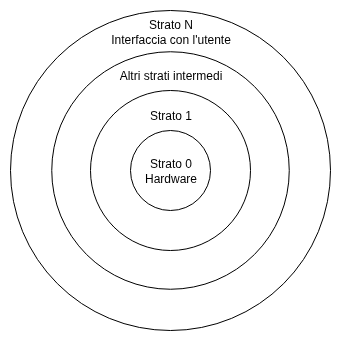
\includegraphics[width=0.5\linewidth]{Images/layered_structure.png}
		\caption{Modello stratificato}	
	\end{figure}
	\item \textbf{Modello repository}: Prevede un componente centralizzato contenente la memoria dei dati e componenti periferici che attuano operazioni di lettura e scrittura in questa memoria. Le periferiche non interagiscono tra loro e parlano esclusivamente con la componente centrale. È adatto ad applicazioni in cui i dati sono prodotti da un sottosistema e usati da un altro, come i case tool, strumenti che aiutano l'ingegneria del software durante il suo ciclo di vita.\par
	Si tratta di un modo efficiente di condividere grandi quantità di dati con una gestione centralizzata del backup e della sicurezza. I sottosistemi dovranno tuttavia accordarsi sulla struttura dei dati per il repository; si tratta di un'evoluzione complessa e costosa, che rende difficile distribuire il software in maniera efficiente.
	\begin{figure}[h]
		\centering
		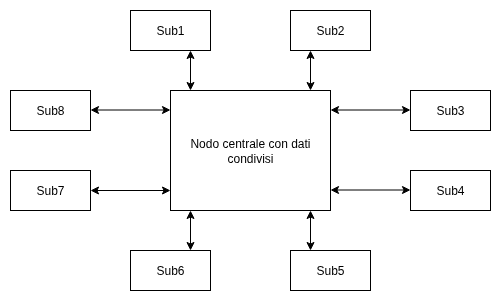
\includegraphics[width=0.8\linewidth]{Images/repository_structure.png}
		\caption{Modello repository}	
	\end{figure}
	\item \textbf{Modello client-server}: Presenta due entità fondamentali; il client, richiedente le informazioni, e il server, che le mantiene e fornisce. La comunicazione tra di loro avviene tramite una rete e le periferiche sono fornite da più server che svolgono appositi job a loro dedicati.\par
	Si tratta di un modello usato normalmente dalle interfacce dei browser web; spostando la computazione tra i vari server si migliorano le prestazioni, il riuso e la mantenibilità. Tuttavia è un sistema distribuito, manca un modello di dati condiviso e il loro scambio può risultare inefficiente per questo. Non è semplice gestire il tutto perché possono presentarsi anche delle ridondanze e alcuni server potrebbero essere prorprietari di un'azienda, quindi al di fuori del proprio controllo.\par
	Esistono due evoluzioni di questo modello; la prima, \textbf{a due livelli}, presenta tre componenti software di \textbf{interfaccia utente}, \textbf{gestione dei processi e logica} e \textbf{gestione del database}, distribuiti sui due strati di client e server. La seconda, presenta \textbf{tre livelli}: uno di \textbf{presentazione}, un secondo per la \textbf{logica} ed il terzo per la \textbf{gestione dei dati}. Il client utilizza esclusivamente l'interfaccia utente, mentre gli altri componenti sono tutti gestiti dal server.
	\begin{figure}[h]
		\centering
		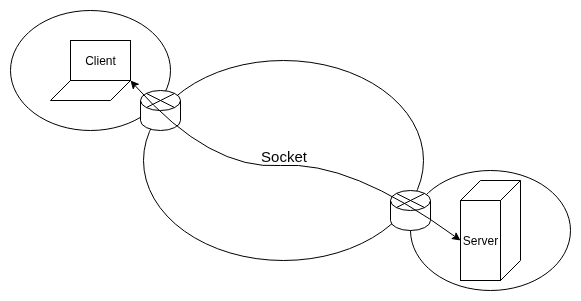
\includegraphics[width=0.8\linewidth]{Images/client-server_structure.png}
		\caption{Modello client-server}	
	\end{figure}
	\item \textbf{Modello peer to peer}: Questa architettura vede ogni componente svolgere il ruolo di client e server mentre esegue il proprio processo. Ogni elemento ha infatti un'interfaccia che specifica i servizi offerti. La comunicazione si basa quindi sulla richiesta e offerta dei servizi.\par
	I sistemi p2p scalano bene grazie alla facilità di inserimento dei nodi nuovi e sono tolleranti ai guasti, perché il "perno" sul quale si regge la struttura è decentralizzato.
	\item \textbf{Modello pipe and filter}: Presenta due entità fondamentali; i filtri, che effettuano trasformazioni sui dati, e i connettori che lo trasmettono ai vari filtri. Si tratta di un sistema che supporta l'esecuzione in parallelo e il riuso delle informazioni. Inoltre, ha un workflow intuitivo, rendendo semplice aggiungere e implementare trasformazioni. Tuttavia, non è adatto a software interattivi, ed è infatti usato spesso nello sviluppo di sistemi batch. Un esempio di questo sistema è il comando grep della bash Unix.
\end{itemize}

%

\section{Modelli di controllo}
Per quanto riguarda il design architetturale, sono presenti anche degli \textbf{stili di controllo} del workflow per decidere come gestire il funzionamento del sistema. Ne esistono due principali: \begin{itemize}
	\item \textbf{Centralizzato}: Un sottosistema ha la responsabilità generale del controllo; avvia e termina gli altri componenti del software.
	\item \textbf{Basato su eventi}: Un sottosistema può rispondere ad eventi generati da altre entità, non esiste quindi un vero e proprio controllore.
\end{itemize}

\noindent L'importanza di conoscere i modelli di controllo risiede nello stesso contesto dei pattern architetturali: la definizione del "come fare" non è completa se si fornisce esclusivamente una visuale astratta del sistema, ragion per cui andiamo nel dettaglio di come sarà gestito il workflow del software: \begin{itemize}
	\item \textbf{Modello call-return}: Presuppone l'esistenza di un sottosistema di controllo (\textbf{Main}) che attiva e cede il controllo ad altri componenti. Decide inoltre l'ordine di esecuzione e, al termine dell'esecuzione della sottocomponente, riprende il controllo del flusso. Si tratta di un modello applicabile esclusivamente a sistemi sequenziali.
	\item \textbf{Modello manager}: Pattern usato quando i sottosistemi possono lavorare in parallelo. Una componente \textbf{manager} controlla avvio, terminazione e coordinamento degli altri processi di sistema. Itera continuamente interrogando interfaccia utente, output ed eventuali sensori per identificare eventi o cambi di stato. Esempi di questo modello sono i sistemi di allarme; il manager interpella costantemente le sottocomponenti, le quali comunicano l'eventuale verificarsi di un dato evento con il segnale acustico.
	\item \textbf{Modello broadcast}: Contrariamente a quanto visto nei precedenti modelli, un componente può annunciare, quindi fare un broadcast, l'esecuzione di uno o più eventi. La trasmissione sarà inviata a tutte le altre entità, ognuna capace di gestirlo, e quelle interessate all'ascolto eseguiranno la procedura associata all'evento. Per questa ragione, un modello tale è chiamato anche \textbf{event-driven}.\par
	I sistemi di sorveglianza utilizzano questo modello, poiché richiedono una costante allerta per gli eventi, la cui segnalazione deve essere comunicata a tutte le apparecchiature in ascolto. È facilmente mantenibile perché risulta semplice aggiungere e rimuovere entità. Tuttavia non è sicuro che l'evento venga gestito da una componente; come conseguenza diretta si potrebbero anche perdere dati importanti durante la trasmissione non ascoltata.
	\item \textbf{Modello a microservizi}: Approccio per lo sviluppo di una singola applicazione come una suite di piccoli servizi, ognuno eseguito nel proprio ambiente e comunicante con gli altri mediante meccanismi semplici, come una API di risorse HTTP. È un modello orientato ai servizi offerti dal software nettamente più mantenibile rispetto ai precedenti, poiché le varie componenti hanno dimensioni ridotte e sono indipendenti l'una dall'altra. Ogni microservizio realizza una funzionalità, possiede le proprie risorse ed è coordinato con gli altri.\par
	Un'altra caratteristica di questo modello è che le varie componenti possono essere scritte in linguaggi di programmazione diversi, perché sono collegati da un gateway\footnote{API Gateway. Si tratta di un design pattern.} per la loro coordinazione.
\end{itemize}
\noindent Arrivati a questa fase del lavoro, si suppone che il design di alto livello, quindi delle specifiche del software e le sue relative interfacce, abbia avuto un riscontro positivo, consentendoci di andare più nel dettaglio e iniziare la \textbf{scrittura delle componenti}. Si determinano le specifiche dettagliate scrivendo interfacce dei singoli elementi che compongono il software, quindi i loro campi, metodi e relazioni necessari per svolgere la propria funzione.\par
Un primo metodo di design per la scrittura di componenti è il \textbf{design by contract}: una progettazione che implementa un \textbf{contratto} tra due entità, il quale deve specificare gli obblighi di entrambe per garantire il loro corretto funzionamento. Si crea un contratto per ogni componente del sistema prima che sia codificata ed è composto da più elementi: \begin{itemize}
	\item \textbf{Pre-condizioni}: Espressioni a valori booleani che rappresenta le aspettative sullo stato del programma prima dell'esecuzione di un'operazione.
	\item \textbf{Post-condizioni}: Espressioni a valori booleani riguardanti lo stato del software dopo l'esecuzione di un'operazione.
	\item \textbf{Invariante di classe}: Condizione che ogni oggetto della classe deve soddisfare in ogni momento in cui è possibile svolgere un'operazione.
\end{itemize}
\noindent Nei contratti si definiscono quindi responsabilità e condizioni da rispettare delle componenti coinvolte; quando queste sono violate, nella pratica viene lanciata un'eccezione. Si definiscono infatti due entità: un \textbf{client}, il cui compito è garantire la validità delle pre-condizioni, e un \textbf{fornitore}, che garantisce la correttezza delle post-condizioni in base alla validità di quanto passato dal client.\par
Questa divisione dei compiti ben specificata è molto utile per vari motivi: in primo luogo, facilita notevolmente il \textbf{debugging}, poiché grazie ai ruoli è possibile ricondursi alla componente che ha lanciato l'eccezione. Se non valgono le pre-condizioni, la colpa sarà del client, mentre se sono violate le post-condizioni il problema sarà situato nel fornitore. In secondo luogo, guida il team nell'implementazione e mantenimento del software, perché presuppone una chiara definizione dei compiti nel contratto, semplificando anche la scrittura degli unit test.\par
In generale, scrivere componenti con il metodo design by contract è molto importante, poiché senza una chiara definizione, si potrebbero effettuare controlli ripetuti delle condizioni in parti diverse del codice, danneggiando le prestazioni con le ridondanze.

%

\section{Principi di progettazione}
Ottenute le specifiche delle singole componenti, si passa alla fase di \textbf{design} delle \textbf{strutture dati} da implementare e \textbf{algoritmi} da utilizzare. Si tratta di un'attività lasciata in gran parte agli sviluppatori e presenta alcune sottofasi: \begin{enumerate}
	\item Analisi del design della classe da scrivere.
	\item Selezione o definizione dell'algoritmo con la relativa notazione.
	\item Scrittura dell'algoritmo mediante \textbf{step-wise refinement}.
	\item Uso dei metodi formali per dimostrare la correttezza del codice.
\end{enumerate}
\noindent Per la notazione degli algoritmi abbiamo a disposizione diversi strumenti, i quali possono essere \textbf{testuali}, come lo pseudocodice, oppure \textbf{visuali}, come diagrammi UML. Prendiamo ora un esempio pratico su cui utilizzare lo step-wise refinement: si inizia con la lettura delle specifiche e si definiscono le dinamiche dell'algoritmo, come i ruoli di client e fornitore insieme ai parametri dei metodi.\par
Dopodiché si passa ad una scrittura più profonda definendo il workflow dei singoli metodi, fino a quando non si è completato l'algoritmo. Lo scopo è ottenere una forma simile alla seguente: \begin{algorithm}[h]
	\caption{getMax(a, b, c)}
	\begin{algorithmic}[i]
		\Require $a$: int, $b$: int, $c$: int
		\State max $\gets$ calcMax(a, b, c)
		\State min $\gets$ calcMin(a, b, c)
		\State res $\gets max-min$
		\State \textbf{return} res
	\end{algorithmic}
\end{algorithm}

\noindent Quello del design è un processo creativo, ma richiede anche dei \textbf{principi di progettazione} per garantire uno standard e guidare lo sviluppo verso il raggiungimento di obiettivi di qualità. Ne esistono molteplici e portano a produrre software mantenibile, comprensibile, semplice da testare, riutilizzabile, portabile e chiaro.\par
Un primo modello è dato dai \textbf{moduli}: entità software identificate da un nome che contiene e fornisce servizi. Presenta un'interfaccia, la parte esternamente visibile, e la parte interna, composta da strutture dati e il codice. I moduli possono interagire fra loro e includerne altri (creando dipendenze); per esempio, in un programma C è possibile definire più file header da includere nel codice.\par
Un'altra idea è l'\textbf{astrazione}, la quale consente di concentrarsi su un problema ad un determinato livello senza perdersi in dettagli di quelli sottostanti. Aiuta a ridurre la complessità e permette di descrivere il comportamento dei moduli più facilmente. Inoltre, nasconde informazioni che gli altri livelli non devono conoscere. Ne esistono diverse forme: \begin{itemize}
	\item \textbf{Funzionale}: Definisce una funzionalità indipendentemente dall'algoritmo che la implementa.
	\item \textbf{Di dati}: Definisce un tipo di dato in base alle operazioni che si attuano su di esso senza definire una struttura concreta.
	\item \textbf{Di controllo}: Definisce un meccanismo di controllo senza mostrare i dettagli interni.
\end{itemize}
\noindent La terza idea è data dalla \textbf{decomposizione}, quindi la partizione di un problema complesso. Conosciuto anche come Divide-et-Impera, consente una più semplice gestione dei problemi in quanto di dimensione ridotta. Impiegando questo principio, tuttavia, sarà necessario spendere anche del tempo per l'integrazione di ogni modulo creato.\par
Una diretta conseguenza della decomposizione è la \textbf{modularità}, un principio che fornisce un criterio detto \textbf{separation of concerns} per la divisione del software: tenere separati gli aspetti che non si riguardano di un software.


% TODO Modularità non è finita



\begin{comment}
	Una valida linea guida è tenere separati il sw di generazione dati dal sw necessario alla presentazione, quindi backend da frontend. Permette di cambiare la rappresentazione dello schermo senza modificare il sistema di calcolo.
	
	Criteri di modularizzazione:
	- Massimizzare coesione e minimizzare l'accoppiamento e dipendenze. Ogni modulo esegue un singolo compito e bisogna minimizzare il numero e la complessità delle interazioni fra i moduli. Consigliato usare delle metriche per vedere quanta complessità è tollerabile in una singola classe.
	
	- Concetto di coesione
	Un modulo coeso svolge un unico compito richiedendo poche interazioni con altri componenti. Usa gli elementi al suo interno lasciando fuori il resto. Permette di comprendere e modificare meglio ogni singolo modulo.
	Ci sono più tipi di coesione: funzionale, di livello, comunicazionale, e altro. L'importante è che seguano la regola di usare le proprie risorse minimizzando il contatto con l'esterno.
	
	- Conceto di accoppiamento
	Ogni modulo non deve dipendere da troppi altri moduli, né dipendervi in modo troppo forte. L'accoppiamento misura il grado di dipendenza di un modulo dali altri. Se ci sono, spesso si richiedono modifiche in più moduli, è difficile capire come un modulo singolo possa lavorare e non si può riutilizzare senza gli altri. È un pò nammerda.
	Capiamo, avere moduli perfettamente indipendenti è irrealistico. Avresti programmi a sé, non un software che li comprende tutti. Allo stesso tempo, non è possibile scrivere dipendenze per tutti i modulo, è disgustosamente difficile da lavorarci. Trova quindi un giusto compromesso, rendendo il software funzionale con il minor numero di dipendenze possibili.
	
	Ci sono diversi tipi di accoppiamento per darci un criterio su quali siano meglio e quali no:
	- Buono: Chiamata di routine, metodo, funzione di altro modulo. Si tratta di una chiamata inevitabile.
	Un altro accoppiamento buono è magari istanziare oggetti di altre classi rendendoli privati e utilizzabili sulla singola classe chiamante (private).
	Anche l'importazione dei componenti non è male.
	- Cattivo: Accoppiamento di contenuto (come componente1 modifica il valore di componente2. I dati dovrebbero essere gestiti da componente2)
	
	- Information hiding
	Moduli dovrebbero essere specificati e progettati sicché le informazioni siano nascoste agli altri moduli ai quali non serve sapere queste informazioni.
	Ogni modulo incapsula una decisione di design separata che potrebbe essere modificata in futuro; le interfacce vengono usate per descrivere ogni modulo in termini delle sue proprietà visibili esternamente.
	Il primo vantaggio di questa strategia è far risultare i moduli debolmente accoppiati grazie alla definizione delle interfacce.
	
	- Alto fan-in, basso fan-out
	Possibile ricostruire il grafo degli usi o dipendenze in cui gli archi rappresentano la relazione di dipendenza. Fan-in sono dipendenze entranti, fan-out sono quelle uscenti. Tanti fan-in indica un buon riuso, mentre tanti fanout indicano eccessiva dipendenza e il modulo dovrebbe essere decomposto.
	
	- Generalità
	Proprietà di design che impatta maggiormente il riuso di un modulo in progetti futuri. Lo scopo è rendere i moduli i più generali possibili per renderlo utilizzabile anche in altri contesti. Per esempio, un algoritmo di ordinamento si usa in molti programmi; generalizzare la procedura per far sì che possa ordinare qualunque parametro non sarebbe male. Rende il codice meno semplice, ma hey, per procedure iperutilizzate va bene.
	
	- Semplicità (DRY KISS, duh)
	
	Esistono delle metriche del software che ci permettono di misurare l'aderenza ai principi visti, come lo IEEE Std 610.12-1990, che è una misura quantitativa del grado di possesso di uno specifico attributo da parte di un sistema, componente o processo.
	Dei tool possono implementarlo, come Stan4J, che funziona a livello di codice.
\end{comment}

%

\section{UML - Unified Modeling Language}
class diagram, use case diagram, activity diagram, sequence diagram

\begin{comment}
	08-04-26 - softEng
	
	--- UML
	Unified modeling language è un linguaggio per il supporto alla descrizione e la progettazione dei sistemi software, tendenzialmente OO. Utile anche per sistemi hardware e capire il dominio del business. Presenta lo standard OMG object management group. Unifica in una collezione di varie notazioni preesistenti, integrate e rese orientate agli oggetti.
	UML è puramente un linguaggio di modellazione, serve solo per esprimere i concetti. Non è usato per programmare.
	
	Con UML si possono fare:
	- abbozzi: aiutano la comunicazione e la discussione, presentando solo le info più importanti. Il tool usato è una lavagna o editor grafici.
	- progetti dettagliati: forniscono un modello completo da implementare usando un UML modeler, come Visual paradigm o papyrus
	- (utilizzato come dei) Linguaggi di programmazione: forniscono un modello eseguibile trasformabile da UML a linguaggio con tool appositi come UniMod o WebRatio
	
	-- Prospettive disponibili
	- Prospettiva software
	Ciò che è descritto nel diagramma sono gli elementi di un sistema software. Per esempio un utente sarà rappresentato come una classe nel linguaggio di programmazione, insieme ai suoi campi. Descrive il design e documenta il software.
	
	- Prospettiva concettuale
	Gli elementi rappresentati sono i concetti del dominio, ed è usato per modellare il dominio del business e i processi.
	
	- Modello di dominio
	Rappresentazione visuale di classi concettuali o di oggetti del mondo reale di un dominio. Si tratta di un glossario visuale delle astrazioni significative del dominio. È utile per chiarire i concetti di dominio per il quale sviluppare il software, ispirare nomi delle classi e degli attributi, ma soprattutto fornisce un punto di partenza per la progettazione del sistema.
	Dalle classi sarà naturalmente possibile rappresentare gli oggetti di dominio; istanze concrete delle classi.
	
	---
	
	UML è uno standard, svolge una funzione di lingua franca, è usato spesso in ambito lavorativo soprattutto per le figure di analista e progettista software.
	UML definisce una famiglia di notazioni e un meta-modello, nel senso che posso descrivere la sintassi UML in UML.
	
	--- Viste, diagrammi e modello
	In UML un sistema è descritto usando diverse viste, intese come un particolare aspetto di un sistema dal punto di vista di un ruolo specifico. Un diagramma descrive una vista e l'insieme dei diagrammi che descrivono gli aspetti del sistema è il modello.
	Disegnamo i modelli con UML 2.0 che contiene 13 tipi di diagrammi. Vedremo i diagrammi use case, class diagram, sequence diagram, activity diagram, state machine diagram e component diagram.
	
	UML può essere usato con qualsiasi processo nelle fasi di raccolta requisiti, design architetturale e delle componenti. È praticamente uno strumento a supporto.
	Nella prima fase possiamo usare uno use case diagram che descrive i requisiti funzionali del sistema dal punto di vista di chi lo usa.
	I diagrammi UML tendenzalmente non sono sufficienti da soli. Esistono due soluzioni per essere esaustivi:
	- cercare o produrre un'estensione di UML (concetto di profilo)
	- Usare diagrammi non UML
	
	-- Mancherebbero le ultime slides, ma nulla di pesante.
\end{comment}
\begin{comment}
	Lez9 - 09-04-26 SoftEng
	
	--- Class diagram
	Definisce classi, le loro feature (attributi e operazioni) e le relazioni tra le classi, come associazioni, aggregazioni/composizioni, specializzazione/generalizzazioni e dipendenze.
	Modelliamo la parte statica (e quindi la struttura) di un sistema software.
	Il significato del diagramma dipende dalla prospettiva, come già detto.
	- concettuale: descriviamo gli elementi del contesto che ci interessa modellare. Una classe è un concetto del dominio e un oggetto è una sua entità. Le operazioni rappresentano le azioni e le responsabilità.
	- software: Descriviamo il design di un software, quindi i moduli che costituiranno l'effettiva implementazione del sistema. Le classi sono le classi in OO, le operazioni sono implementate da metodi.
	
	Il concetto di classe in UML è uguale a quello dell'OO. Tale e quale. Gli oggetti comunicano con scambio di messaggi, pure.
	Rappresentiamo una classe con un rettangolo con il suo nome. In compartimenti sottostanti si indicano gli attributi e le operazioni.
	
	La sintassi per gli attributi è <visibilità nome: tipo [molteplicità] = default{proprietà}>. (default è il valore base dell'attributo di un oggetto appena creato). È possibile anche non visualizzare tutte le informazioni perché possono essere fuorvianti. Di norma basta visibilità, nome e tipo.
	Visibilità indicata come:
	+ pubblico
	- privato
	# protetto
	~ package
	
	Abbiamo nominato la molteplicità: il quantitativo degli attributi (come per esempio le dimensioni per una lista). Alcuni valori possibili sono:
	- 1. Uno singolo, il valore di default
	- 0..1 (al più uno)
	- * Numero imprecisato, eventualmente nessuno, equivalente a 0*
	- 1..* (Almeno uno) // Elementi con molteplicità maggiore di 1 sono considerati un insieme.
	- n..m ed m (m \geq 1)
	
	Anche le operazioni hanno una sintassi: <visibilità nome (parametri): tipo-ritornato {proprietà}>. La lista dei parametri ocontiene nome e tipo dei parametri, secondo la segnatura <direzione nome: tipo = default>.
	La direzione è intesa come input (in), output (out) o entrambi (inout). Il default è input. I getter/setter non sono inseriti, è scontato che ci siano.
	In UML esistono due operazioni:
	- query: ottengono un valore da un oggetto senza side effect
	- modificatori: modificano lo stato dell'oggetto su cui sono chiamate
	
	In UML esiste il concetto di data type che è diverso dagli oggetti. Non sono istanze, non hanno identità; le istanze sono valori in questo caso.
	Degli esempi sono le date o un valore monetario, che hanno senso esclusivamente con i valori. Si indicano specificandoli con lo stereotipo <<datatype>> sopra il nome del tipo.
	
	-- Associazioni
	Un'associazione è una relazione tra le classi. Un -> indica la direzione in cui deve essere letta l'associazione. éer esempio Persona -> automobile indica che la persona possiede l'auto. In alternativa si può indicare il ruolo di uno dei due estremi dell'associazione.
	Puoi indicare questa cosa anche con il verso di navigazione, che indica in quale direzione è possibile reperire le infrmazioni. Con questo, puoi aggiungere anche la molteplicità. È comodo e compatto.
	
	Attributi e associazioni sono due modi per rappresentare la stessa cosa. Per convenzione si usano:
	- attributi per tipi primitivi e datatype
	- Associazioni se sono tipati da classi
	
	--- Object diagram
	Diagramma che consente di rappresentare le istanze di una classe. Considera tutte le possibili combinazioni valide. Servono a chiarire i class diagram più complessi, spiegando anche la relazione tra classe e oggetti con l'operazione <<istanzia>>.
	Le operazioni e i campi static corrispondono esattamente ai metodi e i static types di java. Per indicare che un campo è statico, lo si sottolinea.
	
	- Associazioni riflessive: una classe che ha associazione con sé stessa (parrebbe la relazione ricorsiva dello schema ER)
	- Classi associative
	Talvolta alcune proprietà sono proprie dell'associazione piuttosto che delle classi coinvolte; quindi si aggiunge un rettangolo alla relaizione, al quale è possibile aggiungere attributi e operazioni.
	
	- Asociazioni bidirezionali
	Quando da le informazioni sono recepibili da ambo le direzioni, quindi da entrambe le due classi coinvolte. Non è una cosa implementabile con un singolo attributo e da implementare sono un attimo complesse.
	Nel settare dei valori ad una classe con relazione bidirezionale, così bisognerà fare con l'altra a cui è legato. C'è dunque un problema di sincronizzazione. Per esempio, se ho classi Man e Woman e da una parte setto Man come marito della woman, a sua volta dovrà settare woman come moglie di Man. Per spiegare questo comportamento si esplicita che sono sincronizzate e si aggiunge una nota che specifica il comportamento.
	
	-- Aggregazione
	Altra relazione di tipo strutturale. Si indica con una freccia simil-diamond: regione -<> nazione.
	Una regione è parte di una nazione. Si tratta di una sfaccettatura più importante guardando al livello concettuale, perché a livello software si implementa con un'associazione.
	
	-- Composizione
	Forma più rigorosa di aggregazione. Se il composto è distrutto, così seguiranno le sue parti. È indicato con la diamond-arrow riempita. Le classi aggregate non hanno senso da sole, difatti.
	
	-- Generalizzazione ed ereditarietà
	Per generalizzazione intendiamo che ogni istanza di una classe è anche della superclasse, mentre l'ereditarietà è un meccanismo con il quale elementi specializzati incorporano la struttura ed il comportamento di elementi più generali.
	
	Attenzione che le operazioni e i metodi UML non sono la stessa cosa. Le operazioni sono invocate su oggetti e sono la dichiarazione di una procedura o funzione, mentre un metodo è il CORPO di tale procedura o funzione, quindi la sua definizione.
	
	-- Dipendenze
	Si ha una dipendenza tra due classi se la modifica di una comporta un cambiamento a un'altra.
\end{comment}